\chapter{Regression: Zahlenwerte vorhersagen}
\label{chap:regression}

\begin{myremark}[Algorithmusart in diesem Kapitel]
Funktionsart: \textbf{Regression}. \\
Umsetzungsart: \textbf{selbstlernend}.
\end{myremark}

\begin{myremark}
Dieses Kapitel setzt Kapitel~\cref{chap:einfuehrung} und Kapitel~\cref{chap:datenvorbereitung} voraus.
Regression erweitert das Konzept aus Kapitel~\cref{chap:einfuehrung} (\enquote{Regression}) und zeigt,
wie kontinuierliche Ausgabewerte modelliert werden.
\end{myremark}

\section{Lineare Regression}

\begin{mydefinition}[Lineare Regression]
Die \textbf{lineare Regression} sagt einen kontinuierlichen Zahlenwert $y$ auf Basis
von Merkmalen $x_1, x_2, \ldots, x_n$ vorher:
\[
y = a_0 + a_1 x_1 + a_2 x_2 + \cdots + a_n x_n
\]
Die Koeffizienten $a_i$ werden durch \textbf{Minimierung des quadratischen Fehlers} bestimmt
(Methode der kleinsten Quadrate).
\end{mydefinition}

\begin{figure}[H]
    \centering
    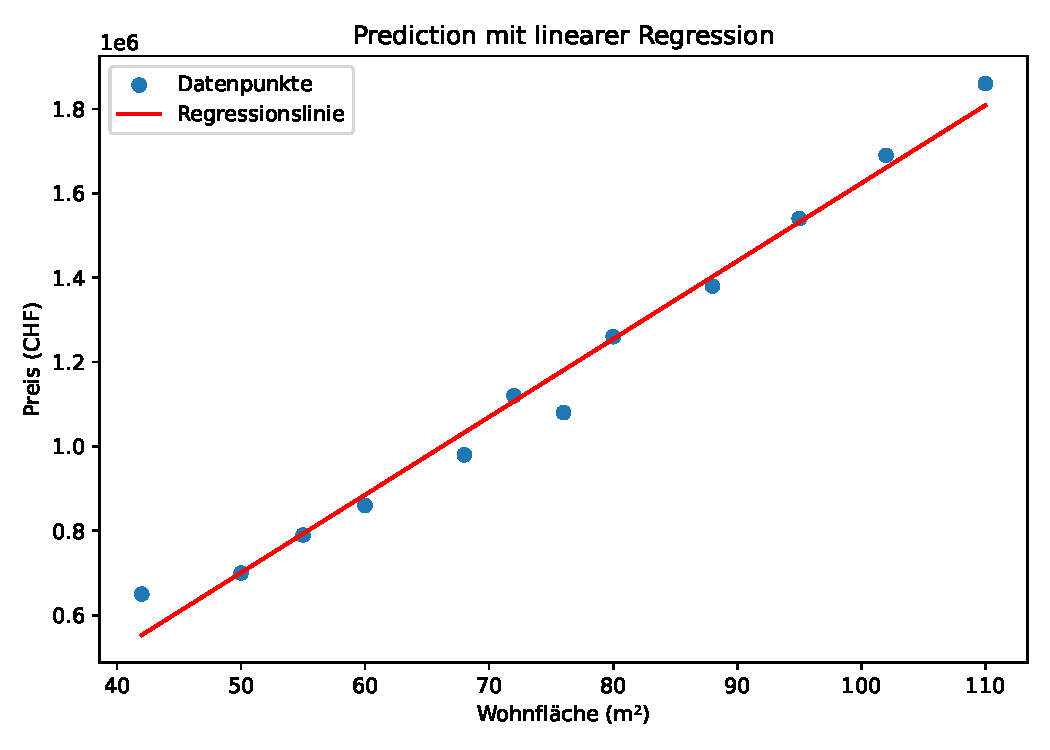
\includegraphics[width=0.75\textwidth]{Grundlagen_Info/10_KI_und_Algorithmen/Figures/regression_prediction.pdf}
    \caption{Lineare Regression: Vorhersage der Wohnungsmiete in Abhängigkeit der Wohnfläche}
    \label{fig:reg-pred-15}
\end{figure}

\section{Interpretation der Koeffizienten}

\begin{myexercise}[Koeffizienten interpretieren]
Ein Regressionsmodell für Wohnungsmieten lautet:
\[
\hat{y} = 500 + 8 \cdot \text{Fläche} - 30 \cdot \text{Stockwerk}
\]
\begin{enumerate}
    \item Was bedeutet der Koeffizient $8$ für die Fläche inhaltlich?
    \item Was bedeutet $-30$ für das Stockwerk? Ist das plausibel?
    \item Wie hoch ist die Vorhersage für eine 60\,m\textsuperscript{2}-Wohnung im 3.\,Stockwerk?
\end{enumerate}
\begin{myanswer}
1.\ Pro m\textsuperscript{2} mehr steigt die Miete um CHF\,8. \\
2.\ Pro Stockwerk höher sinkt die Miete um CHF\,30 (weniger plausibel, eher Datenproblem). \\
3.\ $\hat{y} = 500 + 8 \cdot 60 - 30 \cdot 3 = 500 + 480 - 90 = 890$ CHF.
\end{myanswer}
\end{myexercise}

\section{Gütemasse für Regression}

\begin{mydefinition}[MAE und RMSE]
\[
\text{MAE} = \frac{1}{n}\sum_{i=1}^{n} |y_i - \hat{y}_i|
\qquad\qquad
\text{RMSE} = \sqrt{\frac{1}{n}\sum_{i=1}^{n} (y_i - \hat{y}_i)^2}
\]
\end{mydefinition}

\begin{myexercise}[Fehlermasse vergleichen]
\begin{enumerate}
    \item Welches Mass bestraft grosse Einzelfehler stärker -- MAE oder RMSE?
    \item In welchem Anwendungsfall wäre RMSE besonders sinnvoll?
\end{enumerate}
\begin{myanswer}
1.\ RMSE, weil die Fehler quadriert werden. \\
2.\ Wenn einzelne Ausreisser besonders kritisch sind, z.\,B. bei Energieprognosen für Spitzenlast.
\end{myanswer}
\end{myexercise}

\section{Grenzen der linearen Regression}

\begin{mycaution}
Lineare Regression kann nur \textbf{lineare Zusammenhänge} abbilden.
Bei nichtlinearen Beziehungen (z.\,B. exponentielles Wachstum) sind Erweiterungen wie
\textbf{polynomiale Regression} oder \textbf{Entscheidungsbäume für Regression} nötig.
\end{mycaution}

\begin{mychallenge}[Nichtlineare Daten]
Laden Sie den Datensatz \texttt{apartment\_prices.csv} und fügen Sie ein quadratisches
Feature $\text{Fläche}^2$ hinzu (\emph{Polynomial Features}).
\begin{itemize}
    \item Vergleichen Sie RMSE des linearen und des polynomialen Modells.
    \item Ab welchem Polynomgrad zeigt sich Overfitting?
\end{itemize}
\end{mychallenge}

\section{Gesellschaftliche Aspekte: Regression und Vorhersage-Fehlinterpretationen}

\begin{mydefinition}[Regression sagt nicht die Zukunft voraus]
Ein häufiger Missbrauch: Menschen interpretieren Regressionsmodelle als \enquote{Vorhersage der Zukunft}. Aber Regression findet nur \textbf{historische} Muster. Wenn sich die Bedingungen ändern (z.~B. neue Technologie, wirtschaftliche Krisen), ist die Vorhersage nutzlos -- oder schlimmer noch: irreführend und schädlich.
\end{mydefinition}

\begin{myexample}[Regression in Credit Scoring]
Eine Bank trainiert ein Regressionsmodell auf 20 Jahren historischer Daten. Das Modell sagt Ausfallwahrscheinlichkeiten sehr genau voraus (RMSE = 0.05). Aber:
\begin{itemize}
    \item Diese Genauigkeit gilt nur für Bedingungen ähnlich der Vergangenheit.
    \item Bei einem Schock (z.~B. COVID-19-Pandemie) waren alle Modelle plötzlich nutzlos.
    \item Schlimmer: Die historischen Daten kodieren alte Diskriminierungsmuster. Wer wurde damals als \enquote{risikant} eingestuft? Menschen ohne Kredithistorie, Migranten, Frauen. Das Modell lernt diese Muster und perpetuiert sie.
\end{itemize}
\textbf{Real-World-Fallbeispiel:} \href{https://en.wikipedia.org/wiki/2008_financial_crisis}{Finanzielle Modelle vor der 2008-Krise -- alle waren völlig falsch}
\end{myexample}

\begin{mychallenge}[Vertrauenswürdigkeit vs. Genauigkeit]
Sie sollen ein Modell zur Vorhersage von Hauspreisen entwickeln. Sie haben zwei Optionen:
\begin{itemize}
    \item \textbf{Modell A:} Einfache lineare Regression, RMSE = 45'000 CHF, sehr interpretierbar
    \item \textbf{Modell B:} Neuronales Netz, RMSE = 35'000 CHF, völlig unerklärbar
\end{itemize}
Welches würden Sie für eine Bank empfehlen? Welche Fragen müssten geklärt werden?
\begin{myanswer}
    \begin{enumerate}
        \item \textbf{Makler:} Vielleicht Modell B, weil der Fehler kleiner ist.
        \item \textbf{Hypothekenbank für Privaten:} Modell A ist besser, da Kunden verstehen sollen, warum ihre Schätzung so ist.
        \item \textbf{Was ist die Gewinnspanne?} Ein 10'000 CHF Fehler ist bei 500'000 CHF Häuser negligible, aber kritisch bei 80'000 CHF Häuser.
        \item \textbf{Was passiert bei Modellfehlern?} Wer trägt das Risiko? Das Modell sollte transparent sein, damit klar ist, wer mit dem Fehler leben muss.
    \end{enumerate}
\end{myanswer}
\end{mychallenge}

\begin{myremark}[Notebook]
Praktische Umsetzung inkl. Übungen:
\href{\notebookbaseurl05_Regression_Prediction.ipynb}{\texttt{05\_Regression.ipynb}}
\end{myremark}
